% !TEX root = ../main.tex

% 中英标题:\chapter{中文标题}[英文标题]
\chapter{绪论}[Introduction]

\section{课题研究的背景和意义}[Background, objective and significance of the subject]

地球上的一切都是信号的来源。人类不断测量和收集自然界发生的信号,如温度、风速、降雨量和太阳黑子强度,以适应环境。此外,几十年来,各种各样的工业活动已经在大多数行业领域产生了大量的数据,例如商业(如销售和市场趋势)、金融(如股票价格)、生物医学(如心脏和大脑活动)和制造业(如产量)。在每个行业领域,数据所有者都积极地收集和利用它们来改进产品、流程和服务。特别是,随着工业 4.0 的出现,工业界已经开始密集地利用大量的传感器来同时监测他们的设施和系统,从而提高了效率、安全性\cite{yellow1}。

在各种数据类型中,时间序列数据在医学、气象学和经济学等学术界已经被研究了很长一段时间,时间序列数据现在已经成为大多数实际应用中必不可少的分析对象。时间序列分析是指从时间序列数据中提取有意义的知识的一系列任务,提取的知识不仅可以用来诊断过去的行为,还可以用来预测未来。广为人知的时间序列分析任务包括分类、聚类、预测和异常检测等。其中异常检测任务受到国内外诸多学者的广泛关注\cite{none5, none4, none3, none2, none1}。截至目前,多元时间序列异常检测领域的几个挑战还没有被很好的解决:

\textbf{异常检测召回率低}: 由于异常非常罕见且不均匀,因此很难识别所有的异常。许多正常的实例被错误地报告为异常,而真正复杂的异常被忽略。虽然多年来已经引入了大量的异常检测方法,但是目前最先进的方法,特别是无监督方法(例如\cite{orange17,orange84}) ,仍然经常在现实世界的数据集上引起高度的假阳性\cite{orange20,orange115}。如何减少误报和提高检测召回率是最重要也是最困难的挑战之一,特别是对于不能发现异常的巨大代价。

\textbf{对高维或非独立数据的异常检测}:异常在低维空间中往往表现出明显的异常特征,而在高维空间中则变得隐蔽和不易察觉。高维异常检测一直是一个长期存在的问题。在由一小部分原始特征或自定义特征的简化低维空间中执行异常检测是一个直接的解决方案,例如基于子空间的\cite{orange70,orange77,orange84,orange123}和基于特征选择的方法\cite{orange12,orange109,orange111}。但是,识别复杂的特征(例如,高阶,非线性和异质)相互作用和耦合\cite{orange22}可能在高维数据中是必不可少的,但对于异常检测而言,这仍然是一个主要的挑战。此外,如何保证新的特征空间为特定的检测方法保留适当的信息对于下游的精确异常检测是至关重要的,但是由于上述的未知和异常的不均匀性,这是具有挑战性的。
 
\textbf{对包含缺失值的多元时间序列进行异常检测}:在真实世界中,往往会因为各种非人为因素而导致数据采集不全。例如:传输条件的限制,传感器的自然损坏而没有被及时更换等等而导致数据并数据产生缺失。然而目前并没有方法在包含缺失值的场景下对时间序列进行异常检测。

\section{国内外研究现状}[Developmental of gas-lubricated bearing and correlated theories]

多元时间序列异常检测是识别时间序列数据中异常或意外行为的过程。这是许多领域的一项重要任务,包括金融、网络安全和制造业,因为它使组织能够及时发现和应对潜在问题。多元时间序列异常检测有几种方法,包括统计方法、机器学习方法和基于深度学习的方法。统计方法依赖于分析时间序列数据的统计特性,如平均值和标准差,以识别异常。另一方面,机器学习方法可分为有监督机器学习方法和无监督机器学习方法。其中有监督机器学习方法需要数据集提供明确的正常异常标签,无监督机器学习方法涉及在正常时间序列数据上训练模型,然后使用训练的模型来检测新数据中的异常。同时,深度学习方法是检测时间序列数据异常的有力工具。这些方法基于人工神经网络,可以学习数据中的复杂模式,因此可以用来识别偏离预期行为。近年来,许多学者在发表的综述中对时间序列异常检测相关技术进行了介绍以及总结归纳,本章重点将会对其中基于统计的方法、基于机器学习的方法和基于深度学习的方法的发展历程进行简要阐述,对于其中重点方法的详细技术及细节预计相关知识将在第二章介绍。

\subsection{基于统计学的多元时间序列异常检测研究现状}

统计方法在时间序列异常检测中的应用由来已久。一些最早的方法,如休哈特控制图,是在20世纪20年代和30年代开发的。这些方法依赖于计算时间序列数据的平均值和标准偏差,并使用预定义的规则来识别与预期行为的偏差。随着时间的推移,开发了更复杂的统计方法,如Box-Jenkins\cite{box-jek}方法和自回归综合移动平均(ARIMA)模型\cite{arimax}。这些方法允许对时间序列数据进行更精确的建模,并提高了检测异常的能力。休哈特控制图,也被称为休哈特过程控制图,是由沃特·阿曼德·休哈特在20世纪20年代发展起来的。它是一个图形工具,通过绘制时间序列数据并将其与预定义的上限和下限进行比较,可以监测和控制一个过程。如果数据超出了这些控制范围,则被认为是异常的。Box-Jenkins 方法是由 George Box 和 Gwilym Jenkins 在20世纪70年代开发的一种时间序列数据建模方法。它涉及识别时间序列数据的基本结构,然后拟合该数据的数学模型。这允许更准确地预测未来的值,以及识别异常行为。ARIMA模型模型(ARIMA)是一种统计模型,常用于时间序列分析。它是自回归移动平均(ARMA)模型的一种推广,允许将有关数据趋势和季节性的信息结合起来。这使它成为识别时间序列数据异常的有用工具。

总的来说,这些统计方法已被证明是有效的检测异常的时间序列数据。然而,它们可能很复杂,需要一定程度的专业知识来实现和解释。此外,它们可能并不总是非常适合于处理复杂和动态的系统,在这些系统中,正常的行为没有得到很好的理解,或者正在不断地变化。近年来,统计方法在时间序列异常检测中的应用不断发展。随着大数据的出现和机器学习的进步,越来越倾向于使用更复杂的方法,如机器学习和深度学习。

\subsection{基于机器学习的多元时间序列异常检测研究现状}

基于机器学习的多元时间序列异常检测可以按照是否需要标签分为有监督机器学习方法和无监督机器学习方法。用于时间序列异常检测的有监督机器学习方法是在包含正常和异常行为示例的标记数据集上训练的算法。该算法使用该训练数据来学习数据中指示异常的模式,然后可以应用于新数据以实时识别异常。有许多不同类型的监督机器学习算法可用于时间序列异常检测,包括线性模型、决策树和K近邻。例如Mahmoud等人\cite{none2}首先对时间序列数据进行预处理,以消除所有缺失值,并使用滑动窗口平滑数据。然后,他们从预处理的时间序列数据中提取一系列特征,比如平均值、标准差、最小值、最大值等等。接下来,他们使用这些提取的特征来训练决策树模型。根据时间序列中给定时间点的特征值,训练决策树来预测该时间序列中给定时间点是否为异常。一旦决策树被训练好,它就可以用来对新的时间序列数据进行预测。作者使用决策树中的预测概率来识别可能是异常的时间点,并使用一个阈值来确定哪些点被认为是异常。

有监督机器学习法可以有效地识别时间序列数据中的异常,但也有一些局限性,例如需要对数据进行仔细的预处理,并且无法学习复杂的模式。同时这些算法需要数据集提供标签,当前多元时间序列数据集打标方式大多依赖人工打标,这无疑会给多元时间序列有监督异常检测模型的发展带来挑战。

无监督机器学习方法是检测时间序列数据异常的有力工具。这些方法不需要预先存在的标签,因此可以应用于数据,而无需手动标记。经过多年的发展,时间序列无监督异常检测方法已经发展出许多模式,例如,基于树的方法,基于聚类的方法,基于密度的方法,基于降维的方法等等。孤立森林是一种经典的基于树的异常检测方法,并可以应用到时间序列异常检测中。其由南京大学周志华教授等人提出,是一种从异常点出发,通过指定规则进行划分,根据划分次数进行判断的异常检测方法。该方法对于每个样本点能够根据划分次数计算得到样本异常分数,并根据异常分数与预设阈值的大小比较判断异常;经典的聚类算法,例如K-Means\cite{k-means}或DBSCAN\cite{db-scan}也可用于时间序列异常检测,在这种情况下,算法用于没有任何预先存在的标签的数据,该算法将数据分组成簇,异常被识别为超出预期簇的数据点,这种方法对于检测数据中不符合预期模式的异常非常有用;LOF\cite{LOF}是一种经典的基于密度的检测方法,Gupta等人\cite{lof-app}提出将LOF与聚类算法相结合并应用于时间序列异常检测,LOF 算法计算数据中每个点的局部密度,并使用这种密度来识别与其相邻点明显不同的点,这些点被认为是潜在的异常点,接着作者将聚类算法应用到数据中,将数据点分组成聚类,他们使用聚类通过去除密集聚类中的所有点来细化由 LOF 算法识别的潜在异常集合,最后作者使用一组启发式方法进一步筛选剩余的潜在异常,并确定哪些点被认为是真正的异常。

无论是有监督机器学习方法还是有监督机器学习方法,在时间序列异常检测中使用机器学习方法的一个潜在缺点是它们计算成本可能会很高昂,并且可能需要大量数据来训练模型。这可能使它们不适用于实时应用程序或检测小型或低维数据集中的异常。此外,机器学习模型可能容易过拟合,其中模型在训练数据上表现良好,但不能很好地推广到新的数据。这可能导致假阳性或假阴性异常检测,这在某些应用中可能是昂贵的或有害的。总的来说,虽然机器学习方法对于时间序列异常检测来说是有效的,但是它们也有自己的挑战和局限性。


\subsection{基于深度学习的多元时间序列异常检测研究现状}

深度学习方法已经在多变量时间序列数据的异常检测中显示出有希望的结果。深度学习方法,如递归神经网络(RNN)\cite{RNN, lstm, gru},图神经网络(GNN)\cite{GNN}和对抗生成网络(GAN)\cite{gan}等,特别适合于处理和学习时间序列数据。这些方法可以学习数据中复杂的模式和关系,可以用来建模多变量时间序列数据的时间依赖性和动态。最近的几篇论文\cite{green18, green10, green11, green12}提出了在多变量时间序列数据中使用深度学习方法进行异常检测分析,这些方法已经在各种应用中显示出有希望的结果。一般来说,深度时间序列异常检测模型分为两类,分别对应于基于预测、基于重构的方法。每个类别可以根据之前提到的神经网络技术(RNN、GNN、GAN)进一步划分为子类别。

基于预测的方法值的是使用一个学习好的模型,根据一个点或最近的窗口作为输入,预测下一个点或子序列,将预测值与实际值进行比较,确定传入值的异常程度。它们与实际值的偏差被认为是异常分数。大多数预测方法使用滑动窗口一次预测一个点的方式,为了识别异常行为,他们使用一个预测器来模拟正常行为。这在现实生活中尤其有用,因为在异常检测中,正常行为很多,但异常行为很少。LSTM-NDT\cite{lstm-ndt}提出了一种改进的LSTM模型,通过从多元时间序列中提取历史信息来预测下一个时间步的数据; 同时,文中提出了一种非参数、动态和无监督的阈值搜索技术,可用于评估真是值与预测值之间的残差,通过应用这种方法,可以自动为演化数据设置阈值,以解决多样性、不稳定性和噪声问题。Deng和Hooi\cite{gdn}介绍了GDN,这是一种基于图神经网络注意力的图,通过嵌入向量以捕捉单个传感器的特征,并作为节点,同时捕捉传感器的相关性(空间信息)作为图中的边,学习对其相邻传感器的注意力函数来预测传感器行为。它能够在没有监督的情况下,根据子图、注意力权重以及预测和实际行为的比较,检测和解释与它们的偏差。AD-LTI\cite{ad-lti}是一种预测模型,使用一种名为 Prophet的时间序列分解方法,将 GRU 网络集成在一起,以便能够对没有标签的季节性时间序列数据进行鲁棒学习。通过在运行预测模型之前进行时间序列分解,将输入数据的季节特征明确地反馈到 GRU 网络中。在推理过程中,给出了模型的时间序列及其季节性特征(如周期和日期)。此外,由于预测是基于以前的数据,其中可能包含异常点,他们可能是不可靠的。为了估计异常的概率,它提出了一个新的度量, 称为局部趋势不一致性(LTI)。通过权衡基于最近时间点的帧的预测与其正常的概率,LTI 克服了历史上可能存在异常帧的问题。

基于预测的方法在在在某些场景下可能会失效。大多数复杂的时间序列异常检测方法都是建立在对时间序列建模的基础上,以预测未来的数值和预测误差。即便如此,也没有一个稳健的基于预测的模型可以产生一个快速和不断变化的时间序列的精确模型(见图1-1),因为时间序列在任何给定的时刻都可能是未知的,或者可能像图1-1(b) 那样迅速变化。这样的时间序列无法事先预测,使得基于预测的异常检测无效。基于预测的模型随着时间点数量的增加,预测误差显著增加。由于这个原因,现有的模型作出非常短期的预测,以达到可接受的准确性,因为他们不能检测子序列异常。例如,大多数金融时间序列预测只能预测下一步,如果金融危机可能发生,这是不利的。为了克服基于预测的模型的不足,基于重构的模型可能更有效。

%图片 可预测性,不可预测性
\begin{figure}[htbp]
    \centering
    \subfigure[可预测时间序列]{
    \begin{minipage}[t]{0.5\linewidth}
    \centering
    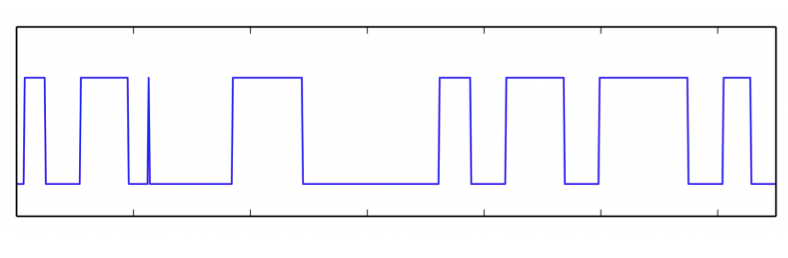
\includegraphics[width=2in]{chapter1/predictable.jpg}
    %\caption{正常时间序列}
    \end{minipage}%
    }%
    \subfigure[不可预测时间序列]{
    \begin{minipage}[t]{0.5\linewidth}
    \centering
    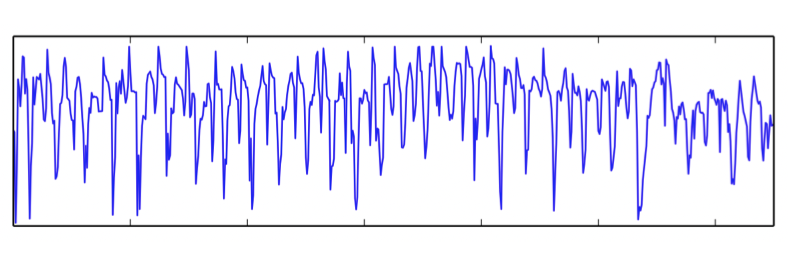
\includegraphics[width=2in]{chapter1/unpredictable.jpg}
    %\caption{数据丢失异常}
    \end{minipage}%
    }%
    \centering
    \caption{可预测时间序列和不可预测时间序列\cite{none1}}
    \end{figure}

基于重建的方法通过在潜在空间(低维)中编码正常训练数据的子序列来构建正常行为的模型。模型输入是滑动窗口,提供重建过程的时间上下文。因为它只在正常数据上训练,所以该模型不可能在测试阶段重建异常子序列。最后,通过从测试数据重建点/滑动窗口并将其与实际值进行比较,检测到异常,称为重建误差。在一些模型中,当重建概率低于指定阈值时触发异常检测,因为异常点/子序列具有低的重建概率。DAGMM(深度自动编码高斯混合模型)\cite{dagmm}在端到端框架中使用潜在空间中的高斯混合先验估计MTS输入样本概率。该模型由两个主要部分组成:压缩网络和估计网络。压缩网络使用随机深度自动编码器对输入样本进行降维,基于降维空间和重建误差特征生成低维表示。估计网络通过低维表示中的高斯混合建模来计算样本能量(定义如下)。样本能量用于确定重建误差;高样本能量意味着高度异常。尽管如此,只考虑空间相关性,不包括时间信息。通过端到端训练,估计网络引入了正则化项,这有助于压缩网络避免局部最优并产生低重建误差。Audibert等人\cite{usad}提出了使用自动编码器的多变量时间序列(USAD)的无监督异常检测,其中使用对抗性训练的自动编码器来放大重建误差。训练或测试的输入是一系列观察结果,这些观察结果具有保留这些信息的时间顺序。此外,对抗性训练加上其架构,使系统能够区分异常,同时促进快速学习。多变量异常检测网络(MAD-GAN)\cite{mtad-gat}是一个基于通用对抗网络(GAN)的模型。该方法利用 LSTM-RNN 作为 GAN 的生成器和鉴别器,同时考虑整个数据,捕捉时间序列分布之间的时间关系, 对于异常检测,采用了重构误差和判别损失两种方法。Goodge等人\cite{apae}通过检查各种对抗性攻击的结果,确定自动编码器在异常检测中是否容易受到对抗性攻击。提出了近似投影自动编码器(APAE),以提高模型在对抗性攻击下的性能和鲁棒性。通过在潜在表示上使用梯度下降,该方法产生了更精确的重建,并提高了对抗性威胁的鲁棒性。同时,加入了特征加权归一化步骤,考虑了不同特征之间重建误差的自然可变性。

\section{本文的主要研究内容}[Developmental of gas-lubricated bearing]

时间序列异常检测是工业界中一个重要的研究领域。并随着近年来越来越多的行业提倡数字化,智能化,吸引了诸多学者进行研究并提出了非常多的多元时间序列异常检测的算法及模型。然而这些方法都是都是面向完整的时间序列数据进行异常检测任务,然而在真实时间中多元时间序列往往包含着大量的缺失值。例如在工业场景中常常因为数据采集不全,传感器损坏等诸多因素所导致时间序列中包含缺失值。故本文课题为缺失值场景下的多元时间序列异常检测,按照填充-检测和不填充-检测的两种思路对包含缺失值的多元时间序列异常检测任务进行了如下研究:

按照填充-检测的思路,本文首先提出了一种基于对抗生成网络的填充算法,并对填充后的多元时间序列进行异常检测。较好的解决缺失值场景下的多元时间序列异常检测任务。本方法通过与多个基线模型对比,在完整数据集上,本章F1分数超过了第二名的基线0.3\%在缺失30\%数据的场景下F1分数超过了第二名的基线3\%,在缺失50\%数据的场景下F1分数超过了第二名的基线5\%。证明了本文的算法在缺失值场景的有效性。

考虑到在填充-检测的解决方案中,模型在训练时需要同时包含缺失值的时间序列和不包含缺失值的时间序列进行学习。这对数据的要求较高,在现实应用中实现难度较大。填充-检测的思路方案依然不能完美的解决缺失值多元时间序列异常检测问题。故本文提出了一种不填充-检测思路的多元时间序列异常检测方案,其基于注意力机制对缺失值时间序列进行重新表征,将不完整的多元时间序列重新表征为完整的高维表征,进而通过对该表征进行异常检测,更鲁棒的解决缺失值场景下的异常检测任务。本方法在三个常用经典时间序列数据集上进行的实验表明,该方法在缺失值场景下对比传统时间序列异常检测方法效果更好。最后,本文通过消融实验验证了各模块的有效性。


\section{论文主要结构与安排}[Main research contents of this subject]
本论文的章节划分安排如下: 第一章是绪论,主要介绍本文的研究背景和意义,面临的挑战以及当前主要的两类异常检测算法研究现状, 在绪论最后总结了本文主要的研究内容。

第二章是缺失值时间序列异常检测技术概述。该章节主要介绍时间序列异常检测技术的基本知识,例如时序数据的异常类型,时间序列的基本属性等;同时介绍了本文所利用到的一些关键技术,例如注意力机制和标准化流技术。

第三章按照填充-检测的思路,首先提出了一种基于对抗生成网络的填充算法,并对填充后的多元时间序列进行异常检测。较好的解决缺失值场景下的多元时间序列异常检测任务。随后通过实验证明本文的算法在缺失值场景的有效性。

第四章按照不填充-检测思路,首先提出了一种基于注意力机制对缺失值时间序列进行重新表征,将不完整的多元时间序列重新表征为完整的高维表征,进而通过对该表征进行异常检测的方案,随后在三个常用经典时间序列数据集上进行的实验表明,该方法在缺失值场景下对比传统时间序列异常检测方法效果更好。最后,本文通过消融实验验证了各模块的有效性。